\documentclass{article}


% if you need to pass options to natbib, use, e.g.:
%     \PassOptionsToPackage{numbers, compress}{natbib}
% before loading neurips_2023


% ready for submission
% \usepackage{neurips_2023}


% to compile a preprint version, e.g., for submission to arXiv, add add the
% [preprint] option:
  \usepackage[preprint]{neurips_2023}


% to compile a camera-ready version, add the [final] option, e.g.:
  % \usepackage[final]{neurips_2023}


% to avoid loading the natbib package, add option nonatbib:
  %  \usepackage[nonatbib]{neurips_2023}


\usepackage[utf8]{inputenc} % allow utf-8 input
\usepackage[T1]{fontenc}    % use 8-bit T1 fonts
\usepackage{hyperref}       % hyperlinks
\usepackage{url}            % simple URL typesetting
\usepackage{booktabs}       % professional-quality tables
\usepackage{amsfonts}       % blackboard math symbols
\usepackage{nicefrac}       % compact symbols for 1/2, etc.
\usepackage{microtype}      % microtypography
\usepackage{xcolor}         % colors
\usepackage{graphicx}       % Required for including graphics
\usepackage{subcaption}     % Required for subfigure environment
\usepackage{listings}       % Required for lstlisting environment
\usepackage{float}          % Enables tables to be rendered anywhere on the page
\usepackage{amsmath}        % For math environments like equation
\usepackage{pgfplots}       % For histogram
\usepackage{tikz}           % For histogram
\pgfplotsset{compat=1.18}


\title{BME1312 Project1 Report: Deep Learning for MRI Reconstruction}


% The \author macro works with any number of authors. There are two commands
% used to separate the names and addresses of multiple authors: \And and \AND.
%
% Using \And between authors leaves it to LaTeX to determine where to break the
% lines. Using \AND forces a line break at that point. So, if LaTeX puts 3 of 4
% authors names on the first line, and the last on the second line, try using
% \AND instead of \And before the third author name.


\author{%
  Wenye Xiong \\
  2023533141 \\
  \texttt{xiongwy2023@shanghaitech.edu.cn}
  \And
  Renyi Yang \\
  2023533030 \\
  \texttt{yangry2023@shanghaitech.edu.cn}
  \AND
  Jiaxing Wu \\
  2023533160 \\
  \texttt{wujx2023@shanghaitech.edu.cn}
  \And
  Boyang Xia \\
  2023533073 \\
  \texttt{xiaby2023@shanghaitech.edu.cn}
  \AND
  Fengmin Yang \\
  2023533183 \\
  \texttt{yangfm2023@shanghaitech.edu.cn}
}

\begin{document}


\maketitle


\begin{abstract}
This report details the implementation and evaluation of U-Net based deep learning models for cardiac segmentation 
in cine MRI scans. The project focuses on segmenting three key structures: the Left Ventricle (LV), Right Ventricle (RV), 
and Myocardium (MYO). We explore the standard U-Net architecture, the impact of removing skip connections, the effect of 
data augmentation, and the performance difference between Cross-Entropy loss and Soft Dice loss.
\end{abstract}

\section{Introduction}
This project aims to:
\begin{enumerate}
  \item Implement a U-Net model for segmenting LV, RV, and MYO from cardiac cine MRI images.
  \item Investigate the role of skip connections in the U-Net architecture.
  \item Evaluate the impact of data augmentation on segmentation performance.
  \item Compare Cross-Entropy loss with Soft Dice loss for training the segmentation model.
\end{enumerate}



\section{Baseline U-Net}

\subsection{Structure}
The U-Net architecture consists of:
\begin{itemize}
  \item \texttt{DoubleConv}: A block of two sequential (Conv2D 3x3, BatchNorm2D, ReLU) operations.
  \item \texttt{Down}: Max pooling (2x2) followed by a \texttt{DoubleConv} block for downsampling in the encoder.
  \item \texttt{Up}: Upsampling (bilinear or transpose convolution) followed by concatenation with features from the 
  corresponding encoder layer (skip connection) and a \texttt{DoubleConv} block. Padding is used to handle potential 
  size mismatches during concatenation.
\end{itemize}

Our baseline is as below:
\begin{itemize}
  \item \textbf{Network}: The standard \texttt{UNet} class as described above, with \texttt{C\_base=32}, 1 input channel, 
  and 3 output classes. Bilinear upsampling was used.
  \item \textbf{Loss Function}: A custom \texttt{MyBinaryCrossEntropy} loss was used. This involves applying a Sigmoid 
  function to the model's output logits to get probabilities, then computing \texttt{nn.BCELoss} against the 3-channel 
  binary ground truth masks. The learning rate was 0.01.
  \item \textbf{Evaluation}: Mean and standard deviation of the Dice Similarity Coefficient (DSC) for LV, RV, and MYO 
  were calculated on the test set. Training and validation loss curves were plotted by the solver. 
  Example segmentation results were saved.
\end{itemize}

\subsection{Experiments and Results}
The training loss and validation loss of the baseline U-Net are shown in figure \ref{fig:baseline_unet_loss}
\begin{figure}[H]
  \centering
  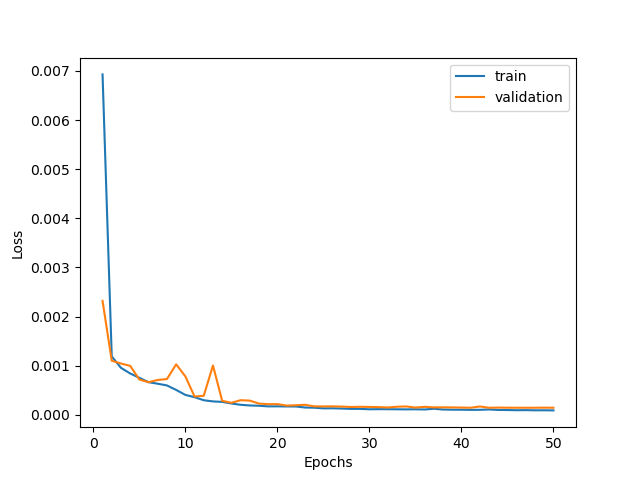
\includegraphics[width=\linewidth]{../result/baseline_unet.png}
  \caption{Training and Validation Loss Curves for the Baseline UNet}
  \label{fig:baseline_unet_loss}
\end{figure}

And here are example segmentation results in figure \ref{fig:baseline_unet_segmentation_example1}, 
\ref{fig:baseline_unet_segmentation_example2}, \ref{fig:baseline_unet_segmentation_example3}
\begin{figure}[H]
  \centering
  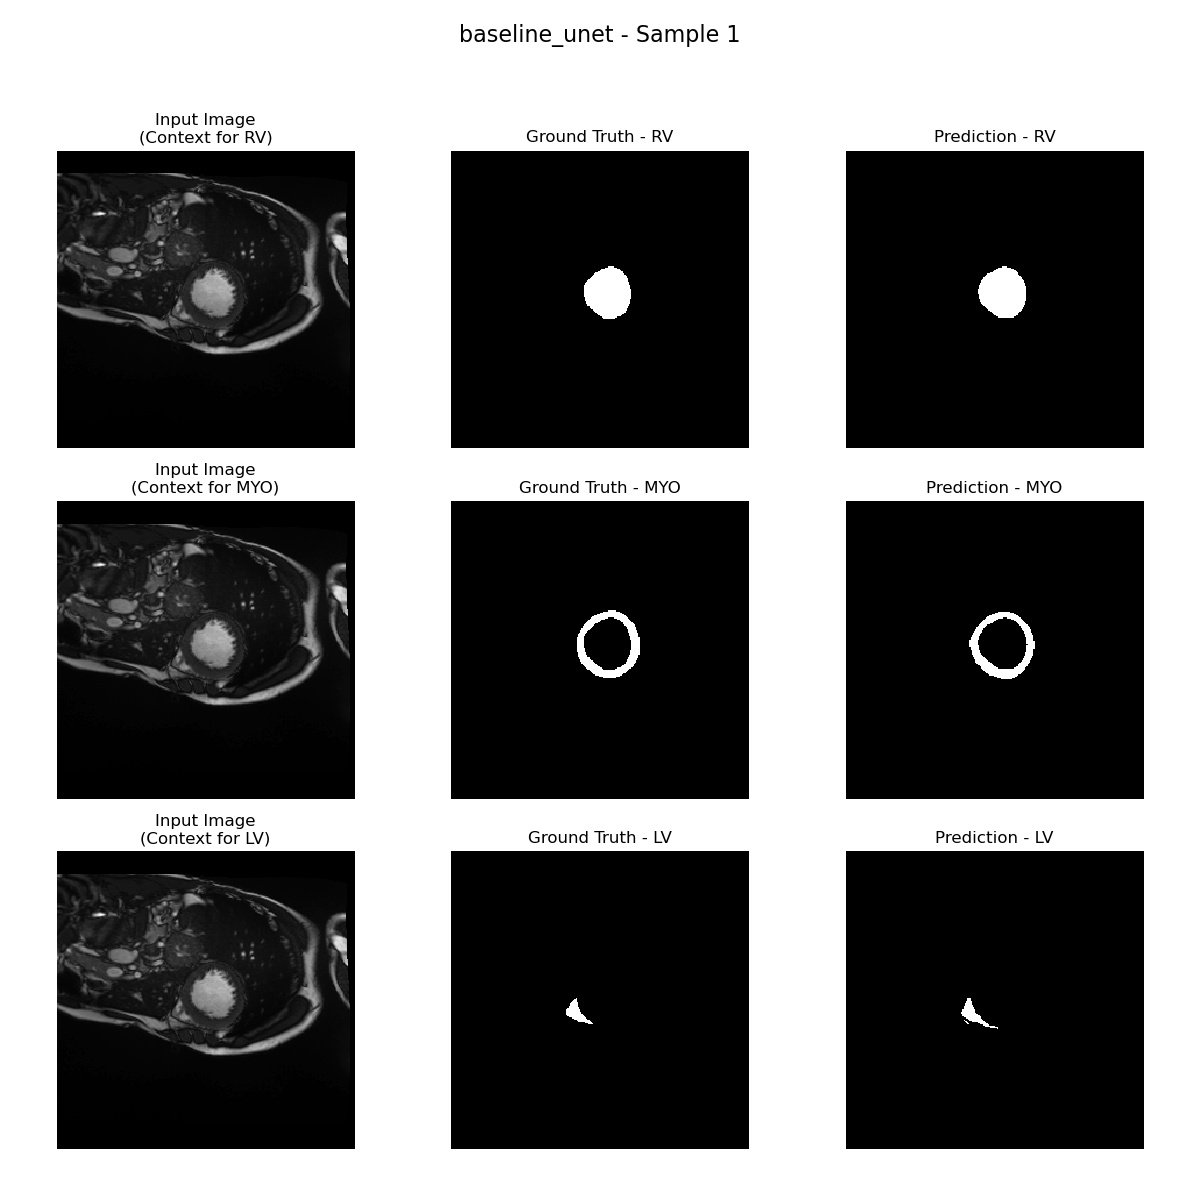
\includegraphics[width=\linewidth]{../result/baseline_unet/sample_1_segmentation.png}
  \caption{An Example Segmentation for the Baseline UNet (1/3)}
  \label{fig:baseline_unet_segmentation_example1}
\end{figure}
\begin{figure}[H]
  \centering
  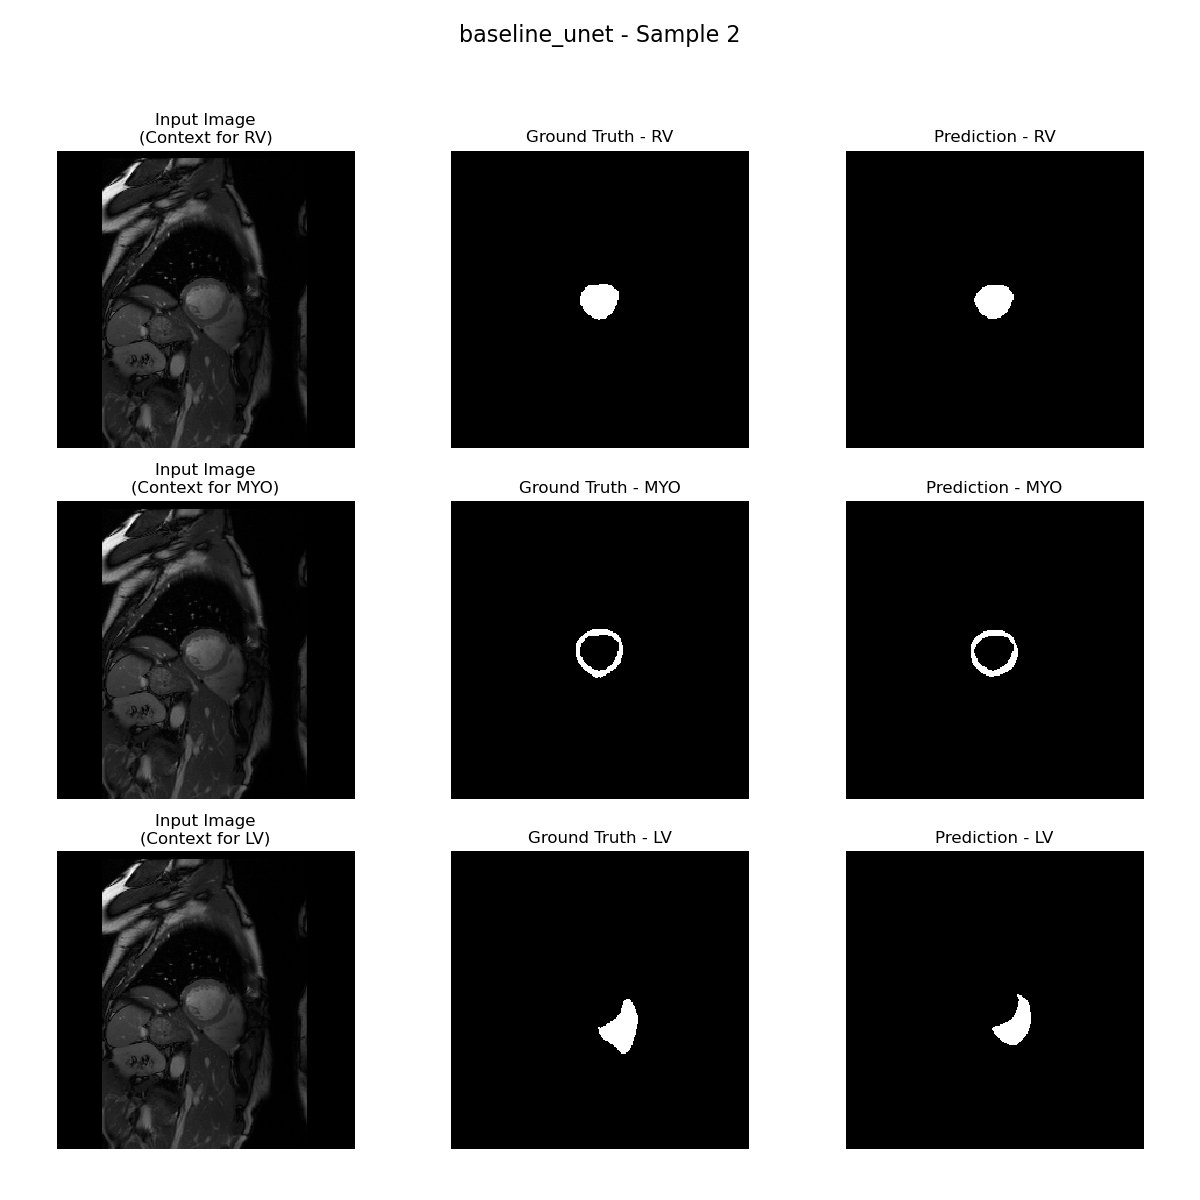
\includegraphics[width=\linewidth]{../result/baseline_unet/sample_2_segmentation.png}
  \caption{An Example Segmentation for the Baseline UNet (2/3)}
  \label{fig:baseline_unet_segmentation_example2}
\end{figure}
\begin{figure}[H]
  \centering
  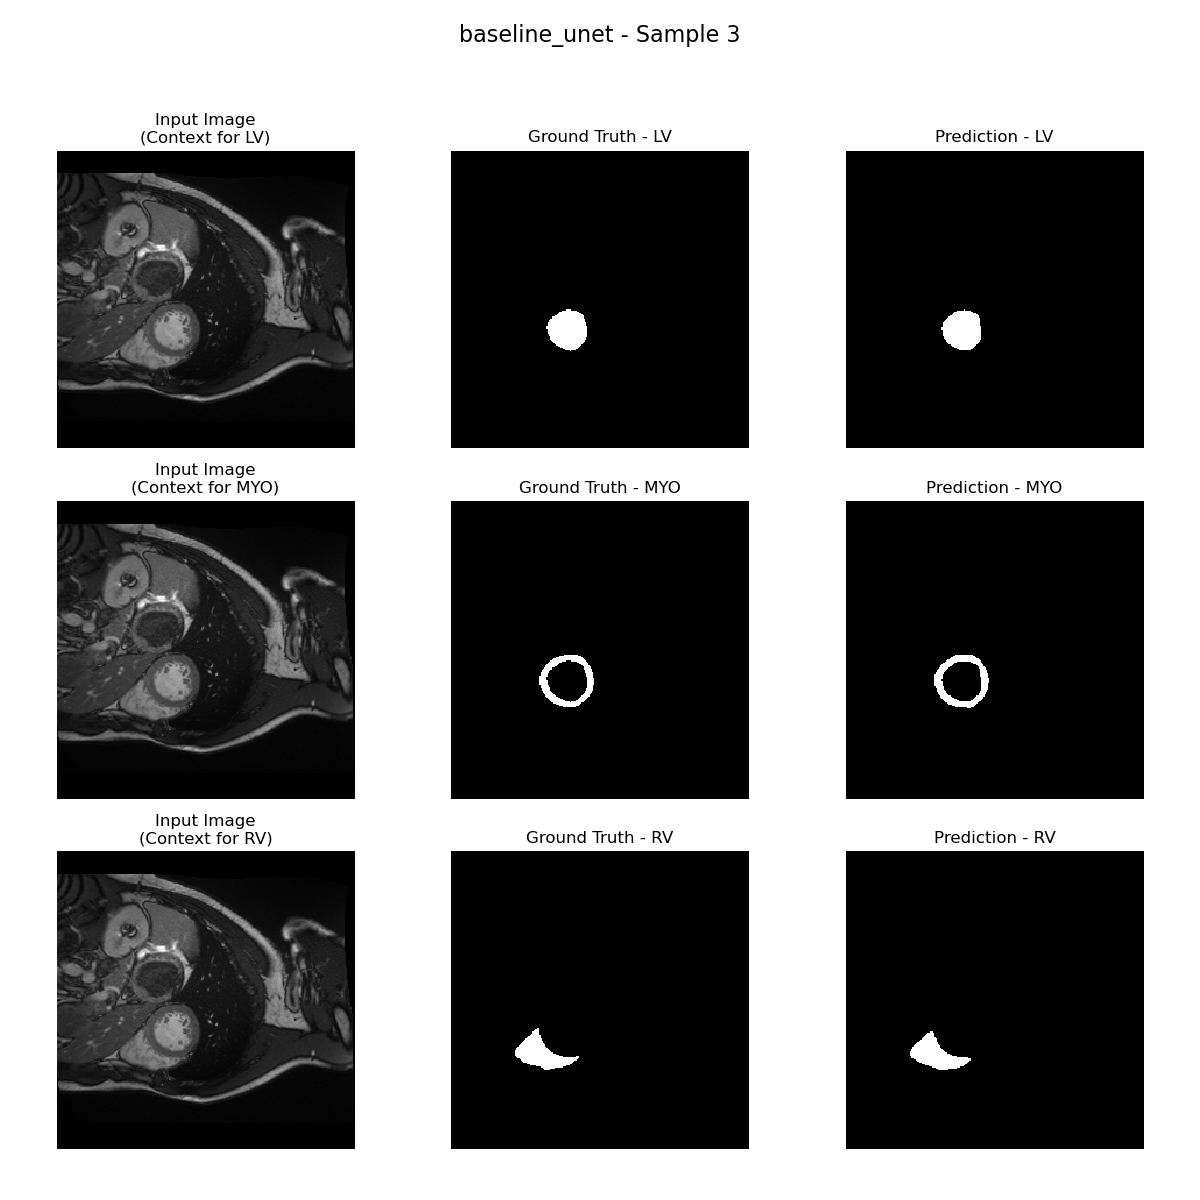
\includegraphics[width=\linewidth]{../result/baseline_unet/sample_3_segmentation.png}
  \caption{An Example Segmentation for the Baseline UNet (3/3)}
  \label{fig:baseline_unet_segmentation_example3}
\end{figure}

The baseline U-Net trained with Cross-Entropy loss achieved the following Dice scores:
\begin{table}[H]
\centering
\caption{Dice Coefficients for Baseline U-Net (Task a)}
\label{tab:baseline_unet}
\begin{tabular}{lcc}
\toprule
Structure & Mean      & Standard Deviation \\
\midrule
RV        & 0.9498    & 0.0089             \\
MYO       & 0.8755    & 0.0120             \\
LV        & 0.8960    & 0.0361             \\
\bottomrule
\end{tabular}
\end{table}

\subsection{Discussion}
The baseline U-Net (Table \ref{tab:baseline_unet}) demonstrated strong segmentation performance.
\begin{itemize}
  \item \textbf{RV Segmentation}: Achieved the highest mean Dice score (0.9498). This is often expected as the RV is 
  typically a large, relatively well-defined structure with good contrast against surrounding tissues in many MRI sequences.
  \item \textbf{LV Segmentation}: Also showed good performance with a mean Dice of 0.8960. The LV cavity is usually clearly visible.
  \item \textbf{MYO Segmentation}: Had the lowest mean Dice score (0.8755). The myocardium is a thinner, more complex structure 
  surrounding the LV, and its boundaries, especially with the LV cavity (endocardium) and epicardium, can be more challenging to 
  delineate accurately, potentially leading to lower overlap scores.
\end{itemize}
The standard deviations are relatively small, indicating consistent performance across the test slices. Overall, the baseline U-Net 
provides a solid foundation for cardiac segmentation.



\section{U-Net without Skip Connections}

\subsection{Structure}
\begin{itemize}
  \item \textbf{Network Modification}: A \texttt{UNet\_NoShortcut} model was implemented. This involved creating an 
  \texttt{Up\_NoShortcut} module that performs upsampling and convolution but does not concatenate features from the encoder 
  path. The \texttt{forward} method of \texttt{Up\_NoShortcut} only processes the feature map from the previous decoder layer.
  \item \textbf{Retraining}: This modified U-Net was trained following the same procedure as the baseline U-Net, 
  including the same dataset split, number of epochs, optimizer, learning rate, and \texttt{MyBinaryCrossEntropy} loss.
\end{itemize}

\subsection{Performance}
The U-Net variant without skip connections, trained under identical conditions, yielded:
\begin{table}[H]
\centering
\caption{Dice Coefficients for U-Net without Skip Connections (Task b)}
\label{tab:no_shortcut_unet}
\begin{tabular}{lcc}
\toprule
Structure & Mean Dice & Standard Deviation \\
\midrule
RV        & 0.9100    & 0.0171             \\
MYO       & 0.8044    & 0.0185             \\
LV        & 0.8499    & 0.0306             \\
\bottomrule
\end{tabular}
\end{table}

\subsection{Discussion}
Comparing Table \ref{tab:no_shortcut_unet} with Table \ref{tab:baseline_unet}, removing skip connections from the U-Net architecture 
resulted in a significant degradation of performance across all three structures:
\begin{itemize}
  \item RV Dice: $0.9498 \rightarrow 0.9100$
  \item MYO Dice: $0.8755 \rightarrow 0.8044$
  \item LV Dice: $0.8960 \rightarrow 0.8499$
\end{itemize}
This substantial drop highlights the critical role of skip connections. Skip connections allow the decoder to reuse high-resolution 
feature maps from the encoder, which contain fine-grained spatial information lost during downsampling. This helps in precise 
localization and reconstruction of segmentation boundaries. Additionally, they facilitate better gradient flow during backpropagation, 
mitigating vanishing gradient problems in deeper networks and aiding convergence. The MYO, being the most intricate structure, 
suffered the largest relative drop in performance.



\section{U-Net with Data Augmentation}

\subsection{Structure}
\begin{itemize}
  \item \textbf{Data Augmentation Techniques}: Augmentations were applied only to the training dataset using 
  \texttt{torchvision.transforms}. A custom \texttt{SegmentationDataset} class was used. In its \texttt{\_\_getitem\_\_} method, 
  the image and its corresponding label (both single-channel tensors) were stacked along a new dimension before applying the 
  transformations. This ensures that geometric augmentations are applied identically to both the image and its mask.
  \item \textbf{Retraining}: The baseline U-Net architecture (with skip connections) was retrained using the augmented training data. 
  The validation set remained un-augmented. The loss function was \texttt{MyBinaryCrossEntropy}, and the learning rate was 0.01.
\end{itemize}

\subsection{Performance}
The baseline U-Net architecture trained with data augmentation on the training set resulted in:
\begin{table}[H]
\centering
\caption{Performance of U-Net with Data Augmentation (Task c)}
\label{tab:data_aug_unet}
\begin{tabular}{l|cc|cc}
\toprule
\multicolumn{1}{c|}{Structure} & \multicolumn{2}{c|}{Accuracy} & \multicolumn{2}{c}{Dice Coefficient} \\
          & Mean      & SD        & Mean          & SD          \\
\midrule
RV        & 0.9988    & 0.0002    & 0.9350        & 0.0109      \\
MYO       & 0.9971    & 0.0003    & 0.8512        & 0.0160      \\
LV        & 0.9978    & 0.0005    & 0.8673        & 0.0353      \\
\bottomrule
\end{tabular}
\end{table}

\subsection{Discussion}
Comparing the Dice coefficients from Table \ref{tab:data_aug_unet} with the baseline U-Net in Table \ref{tab:baseline_unet}:
\begin{itemize}
  \item RV Dice: $0.9498 \rightarrow 0.9350$
  \item MYO Dice: $0.8755 \rightarrow 0.8512$
  \item LV Dice: $0.8960 \rightarrow 0.8673$
\end{itemize}
We can find out that the data augmentation strategy employed led to a slight decrease in Dice coefficients for all structures compared to the 
baseline model trained on un-augmented data. While data augmentation is generally expected to improve generalization and robustness, 
several factors could contribute to this outcome:
\begin{itemize}
  \item 
\end{itemize}
Despite the drop in Dice scores, the pixel-wise accuracy for the augmented model (Table \ref{tab:data_aug_unet}) is very high 
(e.g., RV accuracy 0.9988). However, accuracy can be misleading in segmentation tasks, especially with class imbalance 
(background pixels dominating), whereas Dice is more sensitive to boundary overlap.



\section{U-Net with Soft Dice Loss}

\subsection{Structure}
\begin{itemize}
  \item \textbf{Loss Function Modification}: A \texttt{SoftDiceLoss} class was implemented. This loss calculates the Dice 
  coefficient directly on the sigmoid probabilities of the model's output and the multi-channel binary ground truth. The 
  loss is defined as $1 - \text{mean}(\text{Dice\_per\_class})$. A smoothing factor of 1.0 was added to the numerator and 
  denominator to maintain stability.
  \item \textbf{Retraining}: The U-Net model (same architecture as baseline) was trained using the augmented training 
  dataset (as in Task c) but with the \texttt{SoftDiceLoss}. The learning rate for the Adam optimizer was set to 0.001 for this task.
\end{itemize}

\subsection{Performance}
The U-Net trained with data augmentation and Soft Dice Loss achieved the following pixel-wise accuracies:
\begin{table}[H]
\centering
\caption{Accuracy for U-Net with Soft Dice Loss (Task d)}
\label{tab:soft_dice_unet}
\begin{tabular}{lcc}
\toprule
Structure & Mean Accuracy & Standard Deviation \\
\midrule
RV        & 0.9992      & 0.0001             \\
MYO       & 0.9979      & 0.0002             \\
LV        & 0.9980      & 0.0007             \\
\bottomrule
\end{tabular}
\end{table}

\subsection{Impact of Soft Dice Loss}
The U-Net trained with Soft Dice Loss (and data augmentation) was primarily evaluated using pixel-wise accuracy 
(Table \ref{tab:soft_dice_unet}). Comparing these accuracies to those from the U-Net trained with BCE loss and 
data augmentation (Table \ref{tab:data_aug_unet}):
\begin{itemize}
  \item RV Accuracy: $0.9988 \rightarrow 0.9992 \text{ (Soft Dice)}$
  \item MYO Accuracy: $0.9971 \rightarrow 0.9979 \text{ (Soft Dice)}$
  \item LV Accuracy: $0.9978 \rightarrow 0.9980 \text{ (Soft Dice)}$
\end{itemize}
The Soft Dice Loss resulted in slightly higher pixel-wise accuracies for all structures. This is a positive indication. 
The Soft Dice Loss directly optimizes a surrogate of the Dice coefficient, which is often beneficial for segmentation tasks, 
particularly when dealing with class imbalance, as it focuses on the overlap between prediction and ground truth rather 
than just classifying individual pixels.



\section{Improvement}




\section{Conclusion}
This project successfully implemented and evaluated U-Net based models for cardiac cine MRI segmentation. Key findings include:
\begin{enumerate}
  \item The baseline U-Net provides strong segmentation performance for RV, LV, and MYO, with RV being the best-segmented structure.
  \item Skip connections are essential for U-Net's performance in this task. Their removal led to a significant decline in Dice scores, 
  confirming their importance for feature reuse and precise localization.
  \item The specific data augmentation strategy employed in this study resulted in a slight decrease in Dice coefficients compared to 
  the baseline. This suggests that augmentation parameters need careful tuning and their effectiveness can be dataset-dependent.
  \item Training with Soft Dice Loss yielded slightly higher pixel-wise accuracies compared to Binary Cross-Entropy loss when both 
  were used with data augmentation. This indicates its potential for optimizing segmentation metrics directly.
\end{enumerate}







% \begin{figure}[H]  直方图
%   \centering
%   \begin{tikzpicture}
%     \begin{axis}
%     [ybar, 
%     grid = major, major grid style = {dashed},
%     ymin = 0,
%     ylabel = {SSIM values},
%     title = {SSIM Values for Each Model},
%     bar width = .5cm,
%     width = 40cm,
%     height = 6cm,
%     symbolic x coords={M1, M2, M3, U1, U2, U3},
%     x = 2cm,
%     xtick = data,
%     nodes near coords,
%     nodes near coords style = {font = \fontsize{8}{12}\selectfont},
%     enlarge x limits = 0.2,
%     legend style = {at = {(0.5,-0.2)},anchor = north,legend columns = -1},
%     ] 
%     \addplot+ coordinates {(M1, 0.743) (M2, 0.844) (M3, 0.844) (U1, 0.834) (U2, 0.815) (U3, 0.807)}; 
%     \addplot+ coordinates {(M1, 0.037) (M2, 0.037) (M3, 0.042) (U1, 0.030) (U2, 0.037) (U3, 0.041)}; 
%     \legend{SSIM mean, SSIM std};
%     \end{axis} 
%   \end{tikzpicture}
%   \caption{SSIM Values for Each Model}
%   \label{fig:SSIM Values for Each Model}
% \end{figure}



\end{document}